\documentclass[11pt, a4paper, twoside, table, xcdraw]{report}

%% Language and font encodings
\usepackage[english]{babel}
\usepackage[utf8]{inputenc}
\usepackage[T1]{fontenc}
\usepackage{svg}
\usepackage{listings}
\usepackage{textcomp}

\usepackage{graphicx}
% \usepackage[table,xcdraw]{xcolor}
% If you use beamer only pass "xcolor=table" option, i.e. \documentclass[xcolor=table]{beamer}
\usepackage{lscape}

%% Sets page size and margins
\usepackage[a4paper,top=3cm,bottom=2cm,left=3cm,right=3cm,marginparwidth=1.75cm]{geometry}

%% Useful packages
\usepackage{amsmath}

\usepackage[colorinlistoftodos]{todonotes}
\usepackage[colorlinks=true, allcolors=blue]{hyperref}

\title{Title}
\author{Your Name}


\begin{document}

\begin{titlepage}

\newcommand{\HRule}{\rule{\linewidth}{0.5mm}} % Defines a new command for the horizontal lines, change thickness here

%----------------------------------------------------------------------------------------
%	LOGO SECTION
%----------------------------------------------------------------------------------------
\centering

\includegraphics{./title/Logo20.png}

% Include a department/university logo - this will require the graphicx package

 
%----------------------------------------------------------------------------------------

\center % Center everything on the page

%----------------------------------------------------------------------------------------
%	HEADING SECTIONS
%----------------------------------------------------------------------------------------

\textsc{\LARGE Technical Report}\\[1.5cm] 
\textsc{\Large java group 15}\\[0.5cm] 
\textsc{\large java object oriented programming}\\[0.5cm] 

%----------------------------------------------------------------------------------------
%	TITLE SECTION
%----------------------------------------------------------------------------------------
\makeatletter
\HRule \\[0.4cm]
{ \huge \bfseries Group 15 - Time Scheduler }\\[0.4cm] % Title of your document
\HRule \\[1.5cm]
 
%----------------------------------------------------------------------------------------
%	AUTHOR SECTION
%----------------------------------------------------------------------------------------

\begin{minipage}{0.5\textwidth}
\begin{flushleft} \large
\emph{Authors:}\\
Tim Görß                  - 1252200\\
Ante Maric                - 1273904\\
Minh Triet Huynh          - 1370690\\
Jorge Vanegas Aristizabal - 1333459\\

\end{flushleft}
\end{minipage}
~
\begin{minipage}{0.4\textwidth}
\begin{flushright} \large
\emph{Submitted to:} \\
PhD. Luigi La Blunda \\[1.2em] 
\end{flushright}
\end{minipage}\\[2cm]
\makeatother

%----------------------------------------------------------------------------------------
%	DATE SECTION
%----------------------------------------------------------------------------------------

{\large \today}\\[2cm] % Date, change the \today to a set date if you want to be precise

\vfill % Fill the rest of the page with whitespace

\end{titlepage}


\tableofcontents

% Put all of your chapters here
\chapter{\centering Project Description and Motivation} % Main chapter title

\label{Chapter Project Description} % Change X to a consecutive number; for referencing this 
% chapter elsewhere, use \ref{ChapterX}

Nowadays, time management apps such as Outlook, Google Calendar,etc have proven to be an essential tool in our modern day business and personal lives.

However, the problem with most of these apps is that they require you to have a constant internet connection to use their application. In addition,
the data that you will generate while using these apps belongs to big tech corporations with no clear or transparent way to export it
or to view them outside the app once they are created. These factors along with the fact that the majority of these apps are proprietary 
products mean that they are not an ideal choice for privacy oriented users.

% This is where our project, the time scheduler is born. By combining our Java, database knowledge, and GUI skills we managed to build an app with modern day UI looks that has the ability to create accounts for users and save their information in their locally in their computer. The data store in the computer is only 
% backup in our database if the user choose to do so. In the case that they do, we provide full login, sign up
% functionalities that allow them to continue their work on any machine.

Data protection is a key aspect of our application design. This is why the user's data is backed up in our remote database 
only if they choose to do so by logging in with an existing account or if they sign up for a new account. Otherwise, if they do not want 
their data to be stored in our local database, they can choose to use the offline mode, where all of their data is stored and used locally
on their computer. Both methods have their own way to transfer the data onto another machine allowing the user to be more flexible.  

The main page of the app was designed to offer a modern up-to-date UI that suits the current standards of UI design. Each events and dates 
are color coded in vibrant colors based on their priority so that color blind users can still interact with the app. 

Users are able to create, schedule, edit and delete events, and furthermore invite other users to their event. In addition, our app contains an email function where the users will be reminded to their upcoming event based on the timer option they chose as well as receive emails on upcoming changes or cancellation of event(s) that they are involved in. 

% As mentioned above, privacy is a key feature that we wanted to consider so the data that is generated while using our app can always be exported to either a .txt or database file that can be imported back into the app for later usage. In addition to this, our app can be entirely used without the need for
% any internet connection by using our integrated offline mode.

What is yours will always rightfully belong to you!
% \chapter{\centering Project Description} % Main chapter title

\label{Chapter Project Description} % Change X to a consecutive number; for referencing this 
% chapter elsewhere, use \ref{ChapterX}

This project was created to ease the planning and management of the time spent on activities. It aims to 
increase efficiency and productivity for it's user. Events are visually presented on a live calendar model and 
highlighted based on selected priority, making it faster for the user to distinguish important ones and their 
correlation to others. The data is stored both in a local and in a remote database, so users can access their 
schedule from any PC and even without a internet connection. Events include information about their name, 
description, date, duration, location and participants. Participants added to an event will also receive 
e-mail notifications when changes were made to the event. Admins can use the software to access or delete user
information about e-mail. Admins are able to change the names and e-mails of users.

In addition there is also an offline mode which allows the user to continue working on the database if there is no 
internet connection.

\section{Project Description}


% 
\chapter{\centering Team Organization}
\begin{itemize}
    \item ante maric                - 1273904
    \item tim görß                  - 1252200
	\item jorge vanegas arsitizabal - 1333459
	\item minh triet huynh          - 1370690
\end{itemize}
\chapter{\centering Project Requirements} % Main chapter title

\label{Chapter requierments} % Change X to a consecutive number; for referencing this 
% chapter elsewhere, use \ref{ChapterX}


% Please add the following required packages to your document preamble:
% \usepackage{graphicx}
\begin{table}[h!]
\centering
\resizebox{\textwidth}{!}{%
\begin{tabular}{|l|l|l|l|l|}
\hline
Name &
  Description &
  \begin{tabular}[c]{@{}l@{}}Requirement\\ Type\end{tabular} &
  Actors &
  Member \\ \hline
User sign up &
  \begin{tabular}[c]{@{}l@{}}User are able to create an account \\ with an e-mail and password that \\ is backed up in our remote database\end{tabular} &
  functional &
  User, Admin &
  Triet Huynh \\ \hline
User login &
  \begin{tabular}[c]{@{}l@{}}User can use their associated e-mail and \\ password to log in to their account\end{tabular} &
  functional &
  User, Admin &
  Triet Huynh \\ \hline
Change User information &
  Users can change their e-mail and password &
  non-functional &
  User &
  Jorge \\ \hline
User Setting GUI &
  Users can change settings using a GUI &
  non-functional &
  User &
  Jorge \\ \hline
User Database &
  User data is stored in a database &
  functional &
  User, Admin &
  Triet Huynh \\ \hline
E-mail checker &
  Check if users enter a valid e-mail address &
  non-functional &
  User, Admin &
  Triet Huynh \\ \hline
Password encryption &
  \begin{tabular}[c]{@{}l@{}}Password is stored in our database using \\ a encryption method\end{tabular} &
  non-functional &
  User, Admin &
  Triet Huynh \\ \hline
Login/Registration GUI &
  User can register/login using a GUI &
  functional &
  User,Admin &
  Ante, Triet Huynh\\ \hline
Admin access &
  Admins can login to our software &
  functionall &
  Admin &
  Ante, Triet Huynh\\ \hline
Admin access to user profiles &
  Admins can see all of the user profiles &
  functional &
  Admin &
  Ante \\ \hline
Admin can edit user profiles &
  \begin{tabular}[c]{@{}l@{}}Admins can edit user information such as \\ e-mail and password\end{tabular} &
  functional &
  Admin &
  Ante \\ \hline
Admin can delete user &
  Admins can delete user from database &
  functional &
  Admin &
  Ante \\ \hline
Admin GUI &
  Admin page GUI &
  functional &
  Admin &
  Ante \\ \hline
Create events &
  \begin{tabular}[c]{@{}l@{}}Users are able to create events with \\ specific information\end{tabular} &
  functional &
  User &
  Triet Huynh \\ \hline
Event Database &
  Events are stored in a local database &
  functional &
  User &
  Triet Huynh \\ \hline
Edit events &
  Users can change event information &
  functional &
  User &
  Tim \\ \hline
Delete events &
  Users can delete events &
  functional &
  User &
  Tim \\ \hline
\begin{tabular}[c]{@{}l@{}}E-mail notification when \\ changing events\end{tabular} &
  \begin{tabular}[c]{@{}l@{}}Users that are participants of an event \\ receive an e-mail when changes were \\ made to an event\end{tabular} &
  non-functional &
  User &
  Ante, Tim \\ \hline
Reminder notifications &
  \begin{tabular}[c]{@{}l@{}}Users that are participants of an event \\ receive an e-mail when the reminder \\ is triggered\end{tabular} &
  non-functional &
  User &
  Ante, Tim \\ \hline
Event creation GUI &
  \begin{tabular}[c]{@{}l@{}}Users can use a GUI to create and \\ edit events\end{tabular} &
  functional &
  User &
  Tim, Triet Huynh \\ \hline
Calendar View &
  \begin{tabular}[c]{@{}l@{}}A interact able calendar inside our \\ software to better visualize time\end{tabular} &
  functional &
  User &
  Tim \\ \hline
Events visualized in Calendar &
  \begin{tabular}[c]{@{}l@{}}Events are visualized on a calendar \\ and interact able\end{tabular} &
  functional &
  User &
  Tim \\ \hline
Events highlighted by priority &
  \begin{tabular}[c]{@{}l@{}}Events are highlighted in different colours\\ on our calendar by priority\end{tabular} &
  functional &
  User &
  Tim \\ \hline
Event management GUI &
  Main GUI used for our software &
  functional &
  User &
  Jorge, Tim \\ \hline
Upcoming events &
  \begin{tabular}[c]{@{}l@{}}Upcoming events for the month \\ shown on our GUI\end{tabular} &
  non-functional &
  User &
  Jorge, Tim \\ \hline
Export schedule as plain text file &
  \begin{tabular}[c]{@{}l@{}}Users can export their schedule to a txt file \\ with their local database\end{tabular} &
  non-functional &
  User &
  Triet Huynh \\ \hline
Offline Mode &
  Scheduler is usable without an account &
  non-functional &
  User &
  Triet Huynh \\ \hline
Contact List &
  Participants' emails are stored in the local database &
  functional &
  User &
  Triet Huynh, Jorge\\ \hline
Sync databases &
  \begin{tabular}[c]{@{}l@{}}Users can synchronize their local \\ database with the
  remote database\end{tabular} &
  non-functional &
  User &
  Triet Huynh \\ \hline
\end{tabular}%
}
\caption{Project Requirements and Task distribution table}
\label{tab:requirement}
\end{table}
\chapter{\centering Gantt chart}

% Please add the following required packages to your document preamble:
% \usepackage{graphicx}
% \usepackage[table,xcdraw]{xcolor}
% If you use beamer only pass "xcolor=table" option, i.e. \documentclass[xcolor=table]{beamer}
% \usepackage{lscape}
% \begin{landscape}

\begin{table}[h!]
\centering
\resizebox{\textwidth}{!}{%
\begin{tabular}{|l|l|l|l|l|l|l|l|}
\hline
Tasks &
Week 1 &
Week 2 &
Week 3 &
Week 4 &
Week 5 &
Week 6 &
Week 7
   \\ \hline
\hline
Setting up workplace (IDE, Github, Maven, Overleaf) &
  \cellcolor[HTML]{F8A102} &
   &
   &
   &
   &
   &
   \\ \hline
Drawing diagrams (class diagram, use case diagram) &
  \cellcolor[HTML]{F8A102} &
   &
   &
   &
   &
   &
   \\ \hline
First draft Overleaf documentation (project motivation \& description) & \cellcolor[HTML]{F8A102} &  &  &  &                          &  &  \\ \hline
Creating a database for the user and events &
   &
  \cellcolor[HTML]{FD6864} &
   &
   &
   &
   &
   \\ \hline
Implementing login and sign up function (terminal only) &
   &
  \cellcolor[HTML]{FD6864} &
   &
   &
   &
   &
   \\ \hline
Encryption method for passwords &
   &
  \cellcolor[HTML]{FD6864} &
   &
   &
   &
   &
   \\ \hline
Create GUI for login and sign up &
   &
   &
  \cellcolor[HTML]{986536} &
   &
   &
   &
   \\ \hline
Create event function (terminal only) &
   &
   &
  \cellcolor[HTML]{986536} &
   &
   &
   &
   \\ \hline
Create GUI for events &
   &
   &
   &
  \cellcolor[HTML]{643403} &
   &
   &
   \\ \hline
Create Admin GUI and implement delete/edit functions &
   &
   &
   &
  \cellcolor[HTML]{643403} &
   &
   &
   \\ \hline
Implement calendar functions and Jdate picker &
   &
   &
   &
  \cellcolor[HTML]{643403} &
   &
   &
   \\ \hline
Implement local database and feature to export database &
   &
   &
   &
   &
  \cellcolor[HTML]{036400} &
   &
   \\ \hline
Add participants to events and to friendlist for future events         &                          &  &  &  & \cellcolor[HTML]{036400} &  &  \\ \hline
Create email and reminder function &
   &
   &
   &
   &
   &
  \cellcolor[HTML]{6200C9} &
   \\ \hline
Implement change password for users and its GUI &
   &
   &
   &
   &
   &
  \cellcolor[HTML]{6200C9} &
   \\ \hline
Finish working on the documentation &
   &
   &
   &
   &
   &
   &
  \cellcolor[HTML]{3531FF} \\ \hline
Review everything and fix bugs if needed &
   &
   &
   &
   &
   &
   &
  \cellcolor[HTML]{3531FF} \\ \hline
\end{tabular}%
}
\caption{Gantt Chart}
\label{tab:gantt}
\end{table}
% \end{landscape}

\chapter{\centering Software Description}

\section{GUI}
% Developed by using java Swing but since default does not look appealing, we decided to download a dependency called Flat LaF (look and feel) to change the theme of our overall application making it look more up to date with current application standards.

Initially developed using default java swing, we have decided to use a dependency called \emph{FlatLaf} that allows our application to have aesthetics that is up to date with other current applications' standards, since the look of the default swing framework is rather outdated.

\section{User Registration}

\subsection{Login Page}
The login page is the first page that the user will encounter when they start the app. The page is 
capable of displaying error messages such as: empty email or password field, incorrect email format by using the regex
function to check, and finally display an error message indicating whether the information entered is correct or valid for the user to be
logged in.

\begin{figure}[ht]
	\centering
	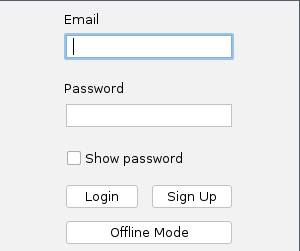
\includegraphics[scale=0.5,keepaspectratio]{Figures/login_page.png}
    \caption{Login page image}
    \label{fig:loginPage}
\end{figure}

Two accounts exist on the remote database that are used purely for testing:
\begin{itemize}
    \item Normal user account email: t@g.com, password: t
    \item Admin user account email: f@g.com, password: f
\end{itemize}

The login page can automatically detect whether the user is an admin or a normal user and redirect them to the corresponding
page.

\subsection{Sign Up Page}
\label{subsection:signup}
If the user is a first time user and doesn't have an account, they can click on the sign up button to be redirected to the sign up page,after which they will be able to create an account by entering an email, password and username. Email and password are required to log into the app and the username will be used to display to other user and in the setting page,this is done because though the email is unique, the username is not, along our user to have a professional and recognizable name to refer to each others. 

If users click on the sign up page by mistake, there is an "already have an account?" button where they can be redirected back to the 
login page.  

An admin account can not be created from the sign up page. But a normal user can be elevate to admin status by an existing admin
using the edit button that they have in their admin page.

\begin{figure}[ht]
	\centering
	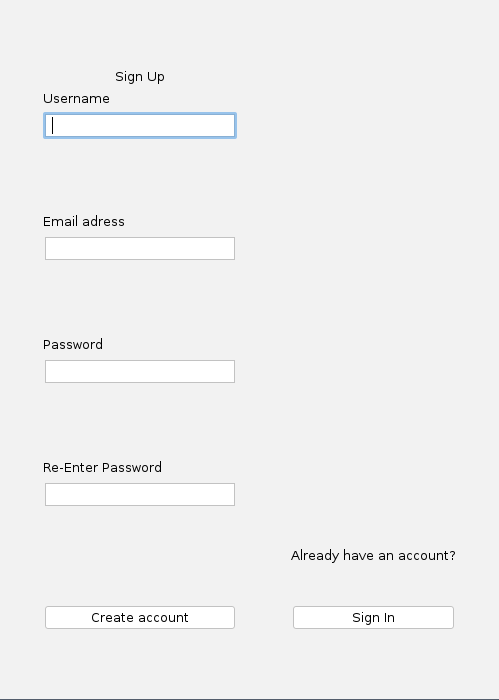
\includegraphics[scale=0.5,keepaspectratio]{Figures/sign_up.png}
	 \caption{Admin page image}
     \label{fig:adminPage}
\end{figure}

\section{Event Page}
Main page of our time scheduler. Here the user has access to most functions of the software.
\subsection{Calendar View}
A live calendar is displayed using the current time of the user's computer as the initial month. Each cell represents a day of the month and can be clicked to open a new frame, showing all events of that day. The cells are highlighted by colours if an event is in our database on that day. The colour changes based on priority from green to red. By clicking the << or >> buttons at the top, the user can change the displayed month of the calendar
\subsection{Side Bar}
Includes a button labeled as "New Event" to access the Add Event page where you can create a new event. The Upcoming Events panel shows you a list of your current events. Lastly the Sync button allows the user to synchronize with the remote database.
\subsection{Adding Events}
A frame allowing to the user to add new events to his scheduler. It can be opened either by using the add event button on the main page or by clicking the add button on the show events page. The user input is checked to avoid invalid inputs.
\subsection{Show Events}
A frame showing all events of single day. It can be opened by clicking on a cell in our calendar. When
an event from the list is clicked, a new frame called Edit Event with additional information about that event is created.
\subsection{Edit Events}
A frame allowing the user to edit information about an event or delete it. It is almost identical in design to the Add Event frame.
\section{Database}
Our application currently operates on two SQL database.
\subsection{Remote}
Database server hosted by Frankfurt UAS faculty 2 for the course Database taught by Prof. Dr. Christian Rich. Connect to the
database using Triet Huynh account assigned to him in the previously mentioned course as learning resource. The database
is using Oracle SQL\texttrademark  and is run constantly 24/7. This is the database that the user interacting with when login,
sign up or use any of the functionalities in the admin page. 

\subsection{Local}
The database is run locally on the user's computer using SQLite version 3036000. SQLite is a light weight implementation of a
DBMS, allowing us to store and retrieve data that doesn't require the user to install anything to be able to interact with the local database. Connection to the local database has almost no latency and is reliable. 
Connection to the local database is only established after the user has finished login or sign up, connection is then terminated when user closed the app.

\section{Security}
\subsection{Password Encryption}
To protect the user from the aftermath of a security breach of our remote server.The user's password is hashed using
sha2-256 locally on the user computer via the application. The remote database only stores the hashed password.

% \subsection{Error message display on incorrect login}
% We decided to show the same error message "Email or password incorrect" in case of the email entered in the login field 
% either does not exist on the remote database and/or is a typo, as well as
% the password entered is incorrect for that account. This is done since an error message i.e. "Account
% with this email address does not exist" would have been displayed at a login try and that will indicate to the malicious hacker or other people that want to 
% gain access to the account the knowledge that the email they have just entered is correct and they now only need to find the correct
% password.

% \subsection{Login page error message}
% The login page will show the same error message both cases if either the user does with that email does not
% exist or the password is entered incorrectly. This is done to provide less information to unauthorized
% people that want to gain access to an account.

% To authenticate the user when they are logging in, the hashed password is then download from the remote database. Then the 
% user entered password from the password field is hashed with the same hash algorithm, the two String is then compare against
% each other.

\section{Admin Page}
The administrator (admin) has extended rights, an individual GUI with a full view/access to the user profiles in the database and executes commands like changing a username or email and the possibility to completely delete a user from the database.  
Admins do not have access to event pages. The admin sole purpose is user database administration.
\subsection{Edit}
The admin has the option to edit the username and/or email of a user if it's i.e. not appropriate and the admin feels that it has to be changed or the user wishes for a name change. The changes will be saved in the database and updated on every other part of the app where the email/username has to be displayed.

\subsection{Delete}
The admin also has the capability to delete a user in case he wants his account deleted for personal reasons or if he has an impression of the user violating the terms of service (i.e. misbehavior, profanity). In case this happens, the user will then be fully deleted and non-existent in the database or application.

\section{Email Function}
The emailUtils class contains all the necessary tools to establish a connection to the gmail servers and a method that is used i.e. to send out predefined automated reminders (depending on the reminder selected) or notifications when events are changed/deleted via user emails passed in as parameters to the participants. It has the option to modify the header/subject and the body (main message) of the email (passed in as parameters as well).

\section{Menu Bar}
The Menu Bar has several drop down menus like Export, About, and most importantly the Menu. There we have the access for the user to the Profile Page, Settings, as well as a Log Out and Exit options.
\subsection{Profile}
The Profile page welcomes the user and displays the superficial details as in username and email but also gives the ID number for each user. Additionally the Profile page shows a Contacts section where the user may enter the Contacts page.
\subsection{Settings}
If the User want change any part of their details, they can make those changes themselves by using the Settings page which offers three methods to change each attribute of the current user.
\subsection{Contacts}
The User has a contact list. This page allows you the options to Add and Delete contacts from your personal contact list. They will then  appear in the add "Participant" tab in the event creation for a day.

\subsection{Database}
% Includes buttons to handle the local database
Include two buttons to export and import the local database.

% \subsubsection{Export Database}
% export the database file to a .db file on the user's computer.

% \subsubsection{Import Database}
% import a SQLite file on the user's computer to be used. The application must be restart for the 
% changes to take effect
\chapter{\centering Diagrams}

\section{Class diagram}
\emph{Author: Jorge Vanegas A. - 1333459\\
Co-Author: Minh Triet Huynh - 1370690}\\
\\The central role is conducted by the User class as it contains the current user information. This is stored in the remote database "DbConnection".
\par To prompt and enter the software the LoginPage will first check the credentials of User from the database, and if they are not registered the SignUpPage then plays the key role in creating a new users and updating the remote database with the new user's data. To be able to gain access to the admin page a check
of the user's credentials similar to one done in Loginpage is also done.
% AdminPage must also check the administrative credentials of the same database. 

\par The only difference is in our local database, implemented to reduce queries latency, and its relationship with the CalendarView, as in our main event. For example there the events are locally stored for ease of access and updates.\\

\chapter{\centering Challenges and Solutions}

During the development of our project, we ran into different challenges as a team and also faced them individually.
In the following section, each member describes their biggest problem(s) and also the solution to it.

% \section{Reduction of boiler plate code}
% \emph{Author Huynh Minh Triet - Matriculation number: 1370690}
% \subsection{Challenge}
% Will building our app following the OOP principle of encapsulation we found out that the majority of 
% the methods in our class are getters and setters, which makes the class extremely long and hard to 
% read.
% \subsection{Solution}
% By using the \emph{Lombok} dependency, all of the getter and setter of the class are automatically 
% generated. Meaning that our team can spend less time on writing repetitive getter, setter code. In addition Lombok allows us to highlight special constructor and getter/setter as these are the only methods that are being shown in the class's code.

\section{Application availability}
\emph{Author Huynh Minh Triet - Matriculation number: 1370690}
\subsection{Challenge}
When first created our app, we did it locally using mySQL hosted locally on Ante's computer. Resulting in the scenario where functions that deal
with the remote database such as: login, sign up or adding events can only be use as long as Ante's personal computer is running. This is
a problem for other team members besides from Ante that want to test with how these database related functionalities work, they are dependent on Ante to get their work done.

\subsection{Solution}
Since one of our team member: Triet Huynh is currently taking the Database course at the same time at the university 
which  supply him a remote database hosted by the university, we decided to use that for our application as a remote 
sever  storing the user's data.

The remote database uses the function sys\_guid() provided by the Oracle database to assign a globally unique ID for
each of the user.This means that no two IDs generated using this method will have the same ID. this function is called
whenever a user has successfully signed up to automatically assign them a unique ID.\\

% Schema of the remote database:
% \begin{lstlisting}[language=SQL]
%  create table UserDB (
%     email    varchar2(100) not null unique,
%     username varchar2(100) not null,
%     hashed_password varchar2(64) not null,
%     user_id raw(16) default sys_guid() constraint 
%     userdb_userid_pk primary key,
%     is_admin number(1) not null,
%     -- This BLOB variable is used to store the local database
%     local_data BLOB 
% )
% \end{lstlisting}


% \section{Multiple connection bug to the remote database}
% \emph{Author Huynh Minh Triet - Matriculation number: 1370690}
% \subsection{Challenge}
% Soon after the usage and deployment of our remote database, we ran into a bug, where due to faulty logical 
% inside the code one instance of the app make continous multiple connection to the remote database. This sudden increase of high volume connection cause the remote database to freeze becoming unresponsive. This results in our application could not be used for a couple of hours. 

% \subsection{Solution}
% We have changed the implementation of the class \emph{DBConnection} that handles the connection to the
% remote database to a singleton class. This makes it impossible for one instance of the app to have multiple 
% connection as a singleton class can only have one object of itself.


\section{Responsiveness and connectivity robustness}
\emph{Author Huynh Minh Triet - Matriculation number: 1370690}

\subsection{Challenge}
At first every interaction with the application that requires stored information is all done through the remote 
database. This cause delay especially when the throughput of the internet connection is slow. Additionally,
the application will come to an abrupt halt if the internet connection is suddenly lost.

Furthermore, the database administrator for the Oracle SQL database that administer the remote server has place a limit 
of one connection to the database for one user account. This problem is discovered when two members of our team tried
to use the application at the same time, wherein they both clicked on the add event button simultaneously causing the 
application to freeze, stopping it from working.

\subsection{Solution}
Though the case mentioned above is relatively rare but we realized that the more each interaction with the application
requires a corresponding query to the remote database the chances of this happening is more often. To solve this
we setup a separate local database using \emph{SQLite} that stores all of the user's data which includes events
and the contact list.

There are three relations that exist on the local database: the event relation, time relation, and participants relation.\\

Additionally a sync button is also added allowing the local database to be uploaded and save in the 
remote database.

\section{Repetitive typing of the participants' emails}
\emph{Author: Huynh Minh Triet - Matriculation number: 1370690: Backend\\
        Co-author    Jorge Vanegas A.- Matriculation number: 1333459: GUI}
\subsection{Challenge}
Earlier version of our application require that each of the participants' emails has to be manually
type in for each events that are being created. While is is feasible for small events with one or two
participants; however, when the number of participants grow to ten or twenty people the chances of typo when 
typing the emails are inevitable. This leads to the reminder not being delivered to the participant and
made the process of adding event a manually intensive and tedious one.

\subsection{Solution}
By adding an additional page to the user's profile page inside setting called  \emph{Contacts}.
Participants can be added into or delete from the contact list store in the local database. 
This contact list is then later shown in the add event page as a scroll panel where the user can 
choose one or multiple participants to add into that event. This allow for frequent participant to be
included with relative ease.


\section{Offline mode}
\emph{Author Huynh Minh Triet - Matriculation number: 1370690}

\subsection{Challenge}
Due to the application not only require the remote database to authenticate the user in login and sign 
up but to also download and upload the local database, the app couldn't be use at all when there
is no internet connection.

\subsection{Solution}
The latest version of the application now has a offline mode which allow the user to use the app 
without any internet connection. When the offline mode is selected and if the application has been
used before, meaning this is not the first time that the user run the application on the current
computer, the application will utilize the current database, allowing them to continue work where
they left off. In the case where this is the first time the application is being run on the machine
a new blank local database will be create.

In addition with the offline button, a new menu bar button called \emph{database}, which when clicked on 
will drop down to reveal two more buttons import and export database; which can be use as backup or to transfer the work onto a different
machine, e.g., you can export the local database to a USB stick and import it later to a different machine.

In the case where internet connection is restored when the user is in offline mode, they can click on the sync 
button which will show the \emph{re-authentication page} where it will ask the user to enter their email and
password to find the account on the remote database. After which they can continue to work in online mode as
usual. The sync button will simply do nothing if internet connection is lost again and the user has to
use the import/export database button to transfer their work. 

\section{Calendar View}
\emph{Author Tim Görß - Matriculation number: 1252200}

\subsection{Challenge}
From the very start of our project we decided against a simple list to display current events of our
users and instead wanted to do a more interact ability and visually pleasing implementation, similar in design to example Google Calendar.


\subsection{Solution}
We use a JTable to display our calendar, where the columns represent the week-days. A Gregorian Calendar object is used to get
the current time of the user and also allow the changing of time. The calendar object also handles leap year problems.
Because each month has a different amount of days and the starting weekdays changes as well, we need more cells than actual days
and create the calendar for each month dynamically.From the first day on wards, the following cells are filled 
with a number according to the days of the month. We use a custom DefaultTableCellRenderer to change the colour of the cells
according to the priority of the events linked to that day. Each cells is also clickable and opens a new frame showing the events
added to that day.

\section{Menu and Side Bar}
\emph{Author Jorge Vanegas A. - Matriculation number: 1333459}

\subsection{Challenge}
As the many features of the application were being added, we found more and more the need to have a place where they could be accessed. For example the Menu which includes Profile, Settings, Exit and Log Out options, as well as Export, Database, and an About page.

\subsection{Solution}
We concurred on the idea to have a fixed side bar, here we could have our sync functions as well as an add event button. Moreover we could show a list of upcoming events to the user. Most importantly however was the implementation of a Menu Bar where all the above mention features could be accessed.

\section{Icons}
\emph{Author Jorge Vanegas A. - Matriculation number: 1333459}

\subsection{Challenge}
GUI with logos and icons would look more pleasing to the user. However we found that Java swing makes it on one side easier to work with the GUI forms, but on the other side a bit more complicated to integrate icons into for example the buttons. Personally could never figure out if it was working with Git or if it was Java swing. We concluded to leave the generic buttons as they are.

\section{Invisible database in JTable}
\emph{Author Ante Maric - Matriculation number: 1273904}

\subsection{Challenge}
While creating the admin GUI that had to display the user database where the admin could edit/delete users from it, the database wouldn't show up in the GUI (empty JTable - invisible database) even though the database was implemented correctly in the code (Tested with System.out.println(); functions).


\subsection{Solution}
After some try and fail options, thoughts about the code being wrong, the solution to it was to manually add the columns and name them above the main section of the actual code to make them visible in the JTable. The database was finally displayed properly and the users could be selected for further function implementation.

\section{Database not updating changes}
\emph{Author Ante Maric - Matriculation number: 1273904}

\subsection{Challenge}
After the admin GUI was created and the database fully displayed and ready to be worked on and after successfully implementing the delete function, we started working on implementing the edit function where the admin can select a user from the database and change his username and/or email. After coding for a while and testing out the implemented SQL queries ("UPDATE XYZ FROM ABC WHERE 123"), the database should be updating the users according to our changes made from the GUI options but it did not. We didn't receive any errors on the execution of the program and the function seemed to work in theory, but as shown in the database it didn't change anything.


\subsection{Solution}
Days have passed and we tried several different changes/options but we didn't get any good results. After additional changes, we received an SQL exception (unique constraint) where it showed us that some attributes in the database where set up to not allow any duplicates with the changes so we had to change them in order to allow the manual edit from our admin panel. As we fixed the database problems, we had to also make some changes to the SQL Queries and combine them with some get methods from our edit function and everything finally updated on the database when we pressed the apply changes button.

\section{Emails not being received and accounts getting banned}
\emph{Author Ante Maric - Matriculation number: 1273904}

\subsection{Challenge}
While testing out the email API, we created some dummy accounts on gmail and tried to send out test emails to see if they were properly sent out and received by our account. The emails were sent out from our program, but there were no emails in the mailbox. 
Email accounts couldn't be used anymore for testing as they were getting banned.


\subsection{Solution}
After some research, we found out that you have to turn ON the "Allow less secure apps to access your account" in the gmail settings to receive the emails on our gmail account. Afterwards, everything worked as it should. After fixing the problem with the receiving emails, the accounts were getting target banned after a few days as they received some test emails and they have been marked as unsafe from gmail as we don't have any licences as other apps/programs have to prove that we are not malicious (problem can't be solved).
\chapter{\centering Conclusion}
\emph{Author Ante Maric - Matriculation number: 1273904}
\newline 

With this project, we had our ups and downs. We learned a lot about team work and trusting each other with the tasks we have been given. If someone struggled and was stuck on a task, there was always someone from the group to speak to/ask for help. This way we grew as a team and had a lot of fun as well working on our project. 

Each and everyone in our group was working hard and faced their own challenges on their way but we all persisted and we are proud of what we have accomplished in this short amount of time.  

We learned a lot of practical things not only in terms of Java and it's functionalities, but also expanded our knowledge on databases, creating GUIs, email API, network connection, understanding the Calendar and time and what can be done with it et cetera. 

Everything we have learned will be of great usage in our future endeavors and we have learned that you have to be adaptive and inventive facing difficulties and changes. 

Never give up and stay persistent, you will eventually overcome your problems and struggles.
\chapter{\centering Sources}

% In this chapter, we will provide information on where we got the code from that might have been used in our project and overall information where we got our ideas/tutorials from.

\section{\emph{Ante Maric - Matriculation number: 1273904}}

\subsection{Email API}
% Good in-depth explanation on how to send emails and how the java mail works overall, a site [1] and a YouTube video tutorial [2]. \newline

\emph{[1]link:} https://www.javatpoint.com/example-of-sending-email-using-java-mail-api 

\emph{[2]link:} https://www.youtube.com/watch?v=A7HAB5whD6I
\newline

\emph{[1]Author:} © Copyright 2011-2021 www.javatpoint.com. All rights reserved. Developed by JavaTpoint.

\emph{[2]Author:} Genuine Coder

\emph{Last accessed:} on the 11th of February, 2022 - 8.11 PM

\subsection{Reminder functionality}
% [1]High quality information on how the Java time and timerTask libraries work and on how to implement them\newline
[2] Youtube tutorial about timers and timerTasks well exlplained\newline

[1]\emph{link:} https://www.baeldung.com/java-timer-and-timertask 

\emph{Author:} Eugen Paraschiv - Baeldung\newline

[2]\emph{link:} https://youtu.be/QEF62Fm81h4 

\emph{Author:} Bro Code\newline

\emph{Last accessed:} on the 11th of February, 2022 - 8.26 PM

\section{\emph{Huynh Minh Triet - Matriculation number: 1370690}}

\subsection{Jfilechooser file type filter}

\emph{link:} https://www.youtube.com/watch?v=lFkYt2jKrYc \newline

% The entire implementation of the class FileTypeFilter.java is copied from the previous youtube video.
% The class allow for the Jfilechooser to only display a certain file type when choosing a file.

\section{\emph{Jorge Vanegas A. - Matriculation number: 1333459}}
\subsection{Menu Bar}
https://www.youtube.com/watch?v=dwLkDGm5EBc \\
\emph{Last accessed:} on the 26th of January, 2022
% https://www.geeksforgeeks.org/java-swing-jmenubar/ \newline
% \par Picked up a few ideas and code from these two links for the JMenuBar and learned how to implement the multiple menus options into our software.



\listoffigures

\end{document}
